\documentclass[aspectratio=169]{beamer}
\usepackage{tikz}
\usepackage{graphicx}

\usecolortheme{whale}
\usetikzlibrary{er,positioning}  
\usetikzlibrary{decorations.pathreplacing}
\usetikzlibrary{arrows, decorations.markings}
\usetikzlibrary{shapes.geometric}

\setbeamertemplate{navigation symbols}{}

\definecolor{violet}{rgb}{0.53, 0.0, 0.69}

\definecolor{blue1}{RGB}{126,126,206}
\definecolor{blue2}{RGB}{87,87,192}
\definecolor{blue3}{RGB}{51,51,178}
\definecolor{blue4}{RGB}{27,26,107}

\tikzstyle{every link} = []
\tikzstyle{link} = [>=triangle 60, draw, every link]

\definecolor{attr}{RGB}{10,153,2}

\title{Bases de Datos}
\subtitle{Ejercitaci\'on. Teor\'ia del dise\~no: Tercera Forma Normal}
\author[Garc\'ia L., Cardentey V. M., Ledesma A.]{
    Lic. Andy Ledesma Garc\'ia\\
    Lic. V\'ictor M. Cardentey Fundora\\ 
    Dra. C. Lucina Garc\'ia Hern\'andez
}
\institute[MATCOM-UH]{
    Departamento de Computaci\'on\\
    Facultad de Matem\'atica y Computaci\'on\\
    Universidad de La Habana\\[3mm]
    Licenciatura en Ciencia de Datos
}
\date[]{15 de febrero de 2024}


\begin{document}
    \maketitle
    % @TODO "previously" frames

\begin{frame}
    \frametitle{Anteriormente... en Bases de Datos...}
    \framesubtitle{Conjunto de entidades e interrelaciones}

    \centering
    \resizebox{!}{7cm}{
    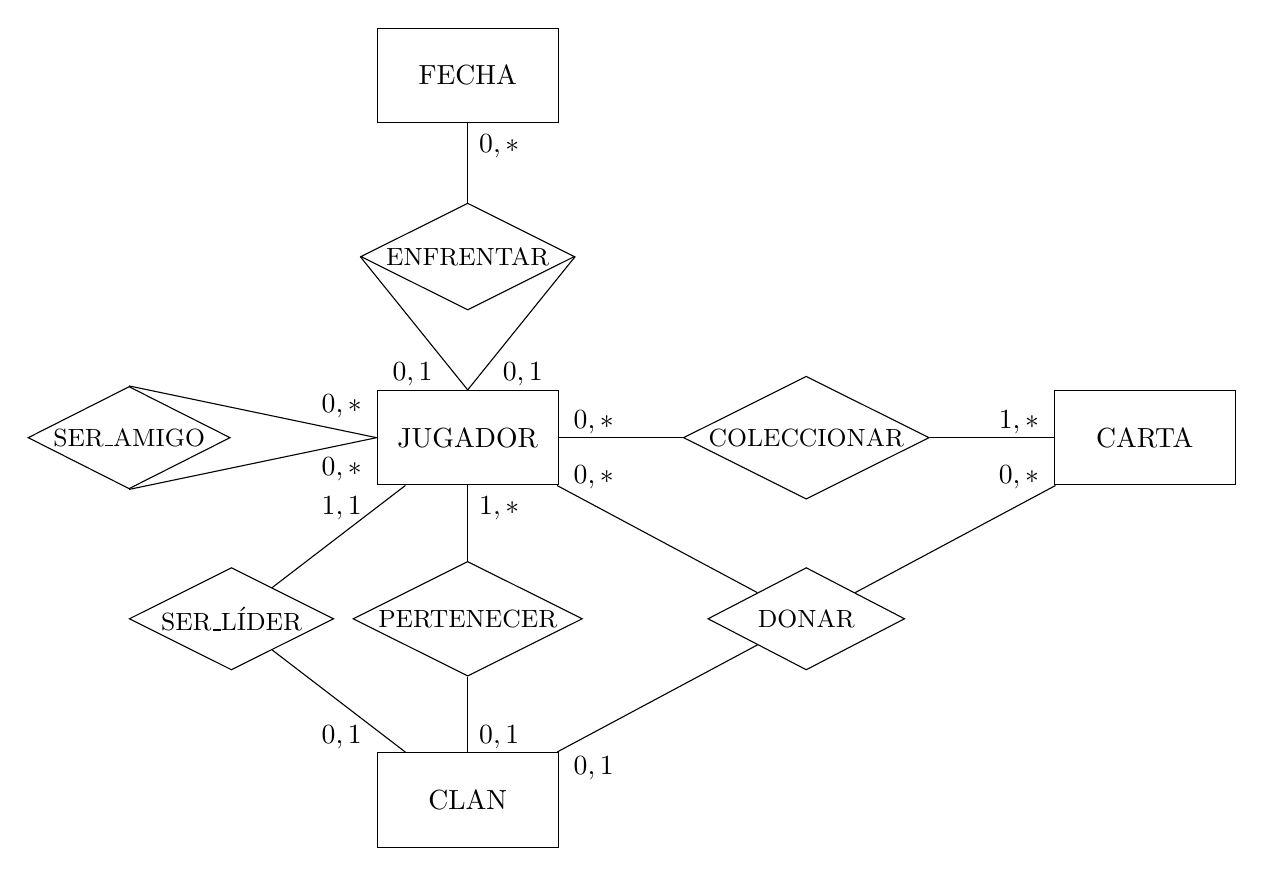
\begin{tikzpicture}
        \tikzstyle{every entity} = [minimum width=2.3cm, minimum height=1.2cm]
        \tikzstyle{every relationship} = [minimum width=2.5cm, minimum height=1.3cm]

        \node[entity] (jugador) at (0,0) {JUGADOR};
        \node[entity] (fecha) at (0,4.6) {FECHA};
        \node[entity] (clan) at (0,-4.6) {CLAN};
        \node[entity] (carta) at (8.6,0) {CARTA};

        \node[relationship,aspect=2] (pertenecer) at (0,-2.3) {\small PERTENECER}
            edge(jugador) edge(clan);
        \node at (0.4,-0.9) {$1,\ast$};
        \node at (0.4,-3.8) {$0,1$};


        \node[relationship,aspect=2] (coleccionar) at (4.3,0) {\small COLECCIONAR}
            edge(carta) edge(jugador);
        \node at (1.6,0.2) {$0,\ast$};
        \node at (7.0,0.2) {$1,\ast$};

        \node[relationship,aspect=2] (enfrentar) at (0,2.3) {\small ENFRENTAR}
            edge(fecha);
        \draw (enfrentar.west) -- (jugador.north);
        \draw (enfrentar.east) -- (jugador.north);
        \node at (0.7,0.8) {$0,1$};
        \node at (-0.7,0.8) {$0,1$};
        \node at (0.4,3.7) {$0,\ast$};

        \node[relationship,aspect=2] (seramigo) at (-4.3, 0) {\small SER\_AMIGO};
        \draw (seramigo.north) -- (jugador.west);
        \draw (seramigo.south) -- (jugador.west);
        \node at (-1.6,-0.4) {$0,\ast$};
        \node at (-1.6,0.4) {$0,\ast$};
      

        \node[relationship,aspect=2] (serlider) at (-3,-2.3) {\small SER\_L\'IDER}
            edge(jugador) edge(clan);
        \node at (-1.6,-3.8) {$0,1$};
        \node at (-1.6,-0.9) {$1,1$};
    

        \node[relationship,aspect=2] (donar) at (4.3,-2.3) {\small DONAR}
            edge(jugador) edge(clan) edge(carta);
        \node at (1.6,-4.2) {$0,1$};
        \node at (1.6,-0.5) {$0,\ast$};
        \node at (7,-0.5) {$0,\ast$};




        
    \end{tikzpicture}
    }

\end{frame}

\begin{frame}
    \frametitle{Anteriormente... en Bases de Datos...}
    \framesubtitle{Atributos}

    \centering
    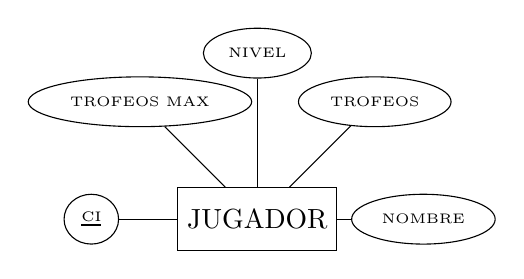
\begin{tikzpicture}[node distance=6em]
        \tikzstyle{every entity} = [minimum width=2cm, minimum height=0.8cm]

        \node[entity] (jugador) {JUGADOR}
            [sibling distance=3cm]
            child {node[attribute] [above left of=jugador] {\tiny TROFEOS MAX}}
            child {node[attribute] [above right of=jugador]{\tiny TROFEOS}}
            child {node[attribute] [above of=jugador] {\tiny NIVEL}}
            child {node[attribute] [right of=jugador]{\tiny NOMBRE}}
            child {node[attribute] (ci) [left of=jugador] {\tiny \underline{CI}}};
    \end{tikzpicture}
\end{frame}
    \begin{frame}
    \frametitle{Ejercicios}
    \framesubtitle<2->{1. Identificando llaves candidatas}
    
    \only<2->{
    Considere la relación $R(U, F)$, tal que 
    $$U = \{A,B,C,D,E\} \quad \textrm{ y } \quad F = \{D \rightarrow C, \ CE \rightarrow A, \ D \rightarrow A, \ AE \rightarrow D \}.$$

    ¿Cuáles de los
    siguientes conjuntos de atributos constituyen llaves candidatas?

    \begin{center}
        CE, BDE, BD, CDE, AD, BCE y A.
    \end{center}

    }

\end{frame}

\begin{frame}
    \frametitle{Ejercicios}
    \framesubtitle{2. Detractores de $E$}

    Considere la relación $R(U, F)$, con $U=\{A,B,C,D,E\}$, que satisface el conjunto de
    dependencias funcionales $F = \{ AB \rightarrow C, \ C \rightarrow D, \ BD \rightarrow E \}$. ¿Cuáles de los siguientes
    conjuntos de atributos no determinan funcionalmente a E?

    \begin{center}
        ABC, AB, BC, AD, ACD, BE y C.
    \end{center}

\end{frame}

\begin{frame}
    \frametitle{Ejercicios}
    \framesubtitle{3. Con $R$ hay que ser legal}

    Suponga que el conjunto universo $U$ de una relación $R$ es $U = \{A,B,C\}$. Actualmente, $R$ s\'olo contiene a la tupla
    $(0,0,0)$, y dicha relación siempre satisface las dependencias funcionales $A \rightarrow B$ y $B \rightarrow C$. ¿Cuáles de las siguientes tuplas pudieran ser insertadas en $R$?
    \begin{center}
        (0,1,0), (0,0,2), (1,1,0), (1,0,2), (0,1,2), (1,2,0) y (1,0,1).
    \end{center}

\end{frame}

\begin{frame}
    \frametitle{Ejercicios}
    \framesubtitle{4. Aprovechando los vac\'ios legales}

    Se conoce de la existencia de una relación $R(U, F)$, donde 

    $$U = \{A,B,C,D,E\} \quad \textrm{ y } \quad F = \{ A \rightarrow B, \ B \rightarrow C, \ DE \rightarrow A \},$$
    pero hemos perdido los valores de ciertas tuplas. ?`Podr\'ias ayudarnos a completarlas? Ten en cuenta que los atributos pueden tomar valores entre 0 y 3.

    \begin{center}
        (0,0,0,1,1), \ (2,1,0,0,3), \ (1,2,0,1,0), \ (1,2, NULL,0,1), \ (3,3,2,0, NULL),\\ (2, NULL, NULL,3,0) 
    \end{center}

\end{frame}

\begin{frame}
    \frametitle{Ejercicios}
    \framesubtitle{5. Aprovechando los vac\'ios legales (la secuela)}

    ¿De verdad entendieron lo que son las dependencias funcionales? Se conoce de la existencia de una relación R(A,B,C,D,E) que satisface las dependencias funcionales:

    $\{ CE \rightarrow A, AE \rightarrow D, A \rightarrow E, D \rightarrow CA \}$

    Pero somos muy despistados y nuevamente hemos perdido valores de ciertas tuplas. ?`Podr\'ias sugerirnos cómo completarlas? Los atributos pueden tomar valores entre 1 y 20.

    %$(2, 1, \gamma, 1, 3), (7, 15, 6, \Delta, 3), (2, 5, \omega, \Omega, \delta), (\alpha, 4, 9, 1, 3)$

    \begin{center}
        (2,1, NULL,1,3), (7,15,6, NULL,3), (2,5, NULL, NULL, NULL),\\
        (NULL,4,9,1,3)  
    \end{center}

\end{frame}
    \begin{frame}
    \centering
    \Huge \textcolor{blue3}{Normalizaci\'on}

\end{frame}
\begin{frame}{Recordar es volver a vivir}

    \resizebox{\linewidth}{!}{
                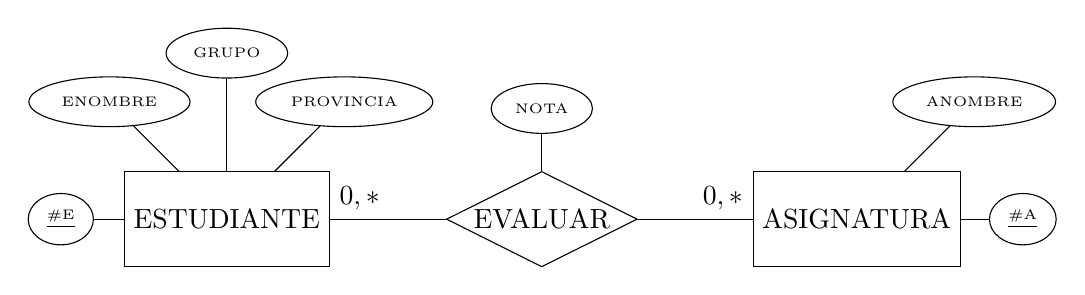
\begin{tikzpicture}[node distance=6em]
                    \tikzstyle{every entity} = [minimum width=2cm, minimum height=1.2cm]
                    \node[entity] (estudiante) {ESTUDIANTE}
                        [sibling distance=3cm]
                        child {node[attribute] [above right of=estudiante] {\tiny PROVINCIA}}
                        child {node[attribute] [above of=estudiante] {\tiny GRUPO}}
                        child {node[attribute] [above left of=estudiante] {\tiny ENOMBRE}}
                        child {node[attribute] [left of=estudiante] {\underline{\tiny \#E}}};
                  
                    \node[entity] (asignatura) at (8,0) {ASIGNATURA}
                    [sibling distance=3cm]
                    child {node[attribute] [right of=asignatura] {\underline{\tiny \#A}}}
                    child {node[attribute] [above right of=asignatura] {\tiny ANOMBRE}};
                    
                  
                    \node[relationship,aspect=2] (evaluar) at (4,0) {EVALUAR}[node distance=4em]
                    child {node[attribute] [above of=evaluar] {\tiny NOTA}};
                    \draw (evaluar.east) -- (asignatura.west) node[above left] {$0,\ast$};
                    \draw (evaluar.west) -- (estudiante.east) node[above right] {$0,\ast$};
                \end{tikzpicture}
            }
\end{frame}
\begin{frame}{¿Es este un buen dise\~no?}
    \centering
    \begin{tabular}{ccccccc}
        \underline{\#E} & ENombre & Grupo & Provincia & \underline{\#A} & ANombre & Nota\\
        $e_1$ & Juan & 111 & La Habana & $a_1$ & An\'alisis & 3\\
        $e_1$ & Juan & 111 & La Habana & $a_2$ & L\'ogica & 2\\
        $e_1$ & Juan & 111 & La Habana  & $a_3$ & \'Algebra & 4\\
        $e_1$ & Juan & 111 & La Habana & $a_4$ & Programaci\'on & 5\\
        $e_3$ & Pedro & 111 & La Habana & $a_3$ & \'Algebra & 4\\
        $e_2$ & Mar\'ia & 112 &  Matanzas & $a_1$ & An\'alisis & 3\\
        $e_2$ & Mar\'ia &  112 & Matanzas & $a_2$ & L\'ogica & 3\\
        $e_4$ & Rita & 112 & Mayabeque & $a_2$ & L\'ogica & 3\\
        $e_4$ & Rita &  112 & Mayabeque & $a_4$ & Programaci\'on & 4\\
        \onslide<-1>{
        $e_5$ & Carlos &  113 & Pinar del R\'io & $a_3$ & \'Algebra & 3
        }
    \end{tabular}
    \vspace{5mm}

    \only<2>{
    \Large
    Anomal\'ias de \textcolor{red}{inserci\'on}, \textcolor{red}{eliminaci\'on} y \textcolor{red}{modificaci\'on}

    }

\end{frame}

\begin{frame}{Entonces...}
    \centering
    \Large ¿C\'omo solucionar estas anomal\'ias?
\end{frame}

\begin{frame}{F\'acil...}
    \begin{columns}[T]
        \begin{column}{0.68\linewidth}
            \begin{columns}[T]
                \begin{column}{0.6\textwidth}
                    \begin{center}
                        \textbf{Estudiante}\\[2mm]
        
                        \begin{tabular}{ccc}
                            \underline{\#E} & ENombre & Provincia\\[1mm]
                            \hline
                            $e_1$ & Juan & La Habana\\
                            $e_2$ & Mar\'ia & Matanzas\\
                            $e_3$ & Pedro & La Habana\\
                            $e_4$ & Rita & Mayabeque\\
                            $e_5$ & Carlos & Pinar del R\'io
                        \end{tabular}
                    \end{center}
                \end{column}

                \begin{column}{0.4\textwidth}
                    \begin{center}
                        \textbf{Provincia-Grupo}\\[2mm]
        
                        \begin{tabular}{cc}
                            \underline{Provincia} & Grupo\\[1mm]
                            \hline
                            La Habana & 111\\
                            Matanzas & 112 \\
                            Mayabeque & 112 \\
                            Pinar del R\'io & 113
                            
                        \end{tabular}
                    \end{center}
                \end{column}
                
            \end{columns}

            \begin{center}
                \textbf{Asignatura}\\[2mm]

                \begin{tabular}{cc}
                    \underline{\#A} & ANombre\\[1mm]
                    \hline
                    $a_1$ & An\'alisis\\
                    $a_2$ & L\'ogica \\
                    $a_3$ & \'Algebra\\
                    $a_4$ & Programaci\'on
                    
                \end{tabular}
            \end{center}
            
        \end{column}

        \begin{column}{0.3\linewidth}
            \vspace{6mm}
            \begin{center}
                \textbf{Evaluar}\\[2mm]

                \begin{tabular}{ccc}
                    \underline{\#E} & \underline{\#A} & Nota\\[1mm]
                    \hline
                    $e_1$ & $a_1$ & 3\\
                    $e_1$ & $a_2$ & 2\\
                    $e_1$ & $a_3$ & 4\\
                    $e_1$ & $a_4$ & 5\\
                    $e_3$ & $a_3$ & 4\\
                    $e_2$ & $a_1$ & 3\\
                    $e_2$ & $a_2$ & 3\\
                    $e_4$ & $a_2$ & 3\\
                    $e_4$ & $a_4$ & 4\\
                    $e_5$ & $a_3$ & 3\\
                \end{tabular}
            \end{center}
        \end{column}
    \end{columns}
\end{frame}

\begin{frame}{Formalizando el dise\~no}
    \centering
    \Large{ ¿C\'omo obtener esta soluci\'on?}
\end{frame}

\begin{frame}{Proyecci\'on de las dependencias funcionales}
    Dados un esquema relacional $R(U,F)$ y un conjunto de atributos
    $Z$ tal que $Z \subseteq U$, la proyecci\'on de un conjunto de dependencias
    funcionales $F$ sobre un conjunto de atributos $Z$ -- denotada
    por $\Pi_Z(F)$ -- consiste en el conjunto de dependencias funcionales
    $X \to Y$ de $F^+$ tales que $XY \subseteq Z$.
    
    $$
        \Pi_Z(F) = \{X \to Y \;|\; F \models X \to Y \land XY \subseteq Z \}
    $$
\end{frame}







\begin{frame}{Descomposici\'on de un esquema relacional}


        %\item $U = \{A_1, A_2,...,A_n\}$  %, $A_i \; (i =1,...,n)$ son atributos
        %simples (Abreviadamente $R = A_1,A_2,...,A_n$)
        La descomposici\'on del esquema relacional $R(U,F)$ se representa por \\[2mm]
        $\rho = \{R_1(U_1,F_1), R_2(U_2,F_2),...,R_n(U_n,F_n)\}$\\[2mm]
        de manera tal que:
        \begin{itemize}
            \item $U = \underset{i = 1}{\overset{n}{\bigcup}} U_i$
            \item Para todo $i = 1,...,n$ se cumple que $F_i = \Pi_{U_i}(F)$ 
        \end{itemize}
\end{frame}


\begin{frame}{Normalizaci\'on de una base de datos relacional}
    \begin{columns}[T]
        \begin{column}{0.48\linewidth}
            \textbf{Estudiante}($U_1$, $F_1$):\\
            $U_1 = \{\textnormal{\#E, ENombre, Provincia}\}$\\
            $F_1 = \{\textnormal{\#E} \to \textnormal{Enombre, Provincia}\}$

        \end{column}

        \begin{column}{0.48\linewidth}
            \textbf{Provincia-Grupo}($U_2$, $F_2$):\\
            $U_2 = \{\textnormal{Provincia, Grupo}\}$\\
            $F_2 = \{\textnormal{Provincia} \to \textnormal{Grupo}\}$
        \end{column}
        
    \end{columns}

    \vspace{10mm}

    \begin{columns}[T]
        \begin{column}{0.48\linewidth}
            \textbf{Asignatura}($U_3$, $F_3$):\\
            $U_3 = \{\textnormal{\#A, ANombre}\}$\\
            $F_3 = \{\textnormal{\#A} \to \textnormal{ANombre}\}$
        \end{column}

        \begin{column}{0.48\linewidth}
            \textbf{Evaluar}($U_4$, $F_4$):\\
            $U_4 = \{\textnormal{\#E, \#A, Nota}\}$\\
            $F_4 = \{\textnormal{\#E, \#A} \to \textnormal{Nota}\}$
        \end{column}
        
    \end{columns}
\end{frame}






\begin{frame}{Formas normales}
    \begin{block}{Primera Forma Normal}
        Un esquema relacional $R(U,F)$ est\'a en primera forma
        normal (1FN) si todos los atributos toman un solo valor del dominio
        subyacente.
        
    \end{block}
\end{frame}

\begin{frame}{La trivial}
    \centering
    \begin{tabular}{ccccccc}
        \underline{\#E} & ENombre & Grupo & Provincia & \underline{\#A} & ANombre & Nota\\
        $e_1$ & Juan & 111 & La Habana & $a_1$ & An\'alisis & 3\\
        $e_1$ & Juan & 111 & La Habana & $a_2$ & L\'ogica & 2\\
        $e_1$ & Juan & 111 & La Habana  & $a_3$ & \'Algebra & 4\\
        $e_1$ & Juan & 111 & La Habana & $a_4$ & Programaci\'on & 5\\
        $e_3$ & Pedro & 111 & La Habana & $a_3$ & \'Algebra & 4\\
        $e_2$ & Mar\'ia & 112 &  Matanzas & $a_1$ & An\'alisis & 3\\
        $e_2$ & Mar\'ia &  112 & Matanzas & $a_2$ & L\'ogica & 3\\
        $e_4$ & Rita & 112 & Mayabeque & $a_2$ & L\'ogica & 3\\
        $e_4$ & Rita &  112 & Mayabeque & $a_4$ & Programaci\'on & 4\\
        $e_5$ & Carlos &  113 & Pinar del R\'io & $a_3$ & \'Algebra & 3
    \end{tabular}
    \vspace{5mm}

    \centering
    \Large \textcolor{red}{Toda relaci\'on se encuentra en primera forma normal}
\end{frame}

\begin{frame}{Dependencia funcional completa}
    Dado un esquema relacional $R(U,F)$ y los atributos $X$, $Y$ de $R$
    (posiblemente compuestos), se dice que $Y$ depende funcional
    y completamente de $X$ si y solo si $Y$ depende funcionalmente de
    $X$ y no depende de alg\'un subconjunto propio de $X$.
\end{frame}

\begin{frame}{¿Qu\'e dependencias funcionales existen en esta relaci\'on?}
    \centering
    \begin{tabular}{ccccccc}
        \underline{\#E} & ENombre & Grupo & Provincia & \underline{\#A} & ANombre & Nota\\
        $e_1$ & Juan & 111 & La Habana & $a_1$ & An\'alisis & 3\\
        $e_1$ & Juan & 111 & La Habana & $a_2$ & L\'ogica & 2\\
        $e_1$ & Juan & 111 & La Habana  & $a_3$ & \'Algebra & 4\\
        $e_1$ & Juan & 111 & La Habana & $a_4$ & Programaci\'on & 5\\
        $e_3$ & Pedro & 111 & La Habana & $a_3$ & \'Algebra & 4\\
        $e_2$ & Mar\'ia & 112 &  Matanzas & $a_1$ & An\'alisis & 3\\
        $e_2$ & Mar\'ia &  112 & Matanzas & $a_2$ & L\'ogica & 3\\
        $e_4$ & Rita & 112 & Mayabeque & $a_2$ & L\'ogica & 3\\
        $e_4$ & Rita &  112 & Mayabeque & $a_4$ & Programaci\'on & 4\\
        $e_5$ & Carlos &  113 & Pinar del R\'io & $a_3$ & \'Algebra & 3
    \end{tabular}
\end{frame}

\begin{frame}{Clasificando dependencias}
    \centering
    \begin{columns}[T]
        \begin{column}{0.2\linewidth}
            
        \end{column}
        \begin{column}{0.3\linewidth}
            {\color<2>{blue}
            \#E, \#A $\to$ ENombre\\
            \#E, \#A $\to$ Grupo\\
            \#E, \#A $\to$ Provincia\\
            \#E, \#A $\to$ ANombre\\
            \vspace{1mm}
            }
            {\color<2>{orange}
            \#E, \#A $\to$ Nota\\
            \#E $\to$ ENombre\\
            \#E $\to$ Grupo\\
            \#E $\to$ Provincia\\
            \#A $\to$ ANombre\\
            Provincia $\to$ Grupo
            }
        \end{column}
        \begin{column}{0.3\linewidth}
            \onslide<2>{
            \vspace{5mm}
            \textcolor{blue}{\Large Incompletas}

            \vspace{20mm}
            \textcolor{orange}{\Large Completas}
            }
        \end{column}
        \begin{column}{0.2\linewidth}
            
        \end{column}
    \end{columns}
        
\end{frame}

\begin{frame}{Formas normales}
    \begin{block}{Segunda Forma Normal}
        Un esquema relacional $R(U,F)$ est\'a en segunda
        forma normal (2FN), si est\'a en 1FN y todos los atributos
        no llaves dependen completamente de la llave.
        
    \end{block}
\end{frame}


\begin{frame}{Llegando hasta segunda}
    \vspace{-5mm}
    \begin{columns}[T]
        \begin{column}{0.68\linewidth}
            \begin{center}
                \textbf{Estudiante}\\[2mm]

                \begin{tabular}{cccc}
                    \underline{\#E} & ENombre & Provincia & Grupo\\[1mm]
                    \hline
                    $e_1$ & Juan & La Habana & {\color<2>{red}111}\\
                    $e_2$ & Mar\'ia & Matanzas & 112\\
                    $e_3$ & Pedro & La Habana & {\color<2>{red}111}\\
                    $e_4$ & Rita & Mayabeque & 112\\
                    $e_5$ & Carlos & Pinar del R\'io & 113\\
                \end{tabular}
            \end{center}
            

               

            \begin{center}
                \textbf{Asignatura}\\[2mm]

                \begin{tabular}{cc}
                    \underline{\#A} & ANombre\\[1mm]
                    \hline
                    $a_1$ & An\'alisis\\
                    $a_2$ & L\'ogica \\
                    $a_3$ & \'Algebra\\
                    $a_4$ & Programaci\'on
                    
                \end{tabular}
            \end{center}
            
        \end{column}

        \begin{column}{0.3\linewidth}
            \vspace{6mm}
            \begin{center}
                \textbf{Evaluar}\\[2mm]

                \begin{tabular}{ccc}
                    \underline{\#E} & \underline{\#A} & Nota\\[1mm]
                    \hline
                    $e_1$ & $a_1$ & 3\\
                    $e_1$ & $a_2$ & 2\\
                    $e_1$ & $a_3$ & 4\\
                    $e_1$ & $a_4$ & 5\\
                    $e_3$ & $a_3$ & 4\\
                    $e_2$ & $a_1$ & 3\\
                    $e_2$ & $a_2$ & 3\\
                    $e_4$ & $a_2$ & 3\\
                    $e_4$ & $a_4$ & 4\\
                    $e_5$ & $a_3$ & 3\\
                \end{tabular}
            \end{center}
        \end{column}
    \end{columns}
\end{frame}

\begin{frame}{Llegando hasta segunda}
    \centering
    \Large \textcolor{red}{Todav\'ia existe redundancia innecesaria}
\end{frame}

\begin{frame}{Dependencia funcional transitiva}
    Dado un esquema relacional $R(U,F)$ y los atributos $X$, $Y$ y $Z$ de
    $R$ (posiblemente compuestos), se dice que $Z$ depende funcional
    y transitivamente de $X$ si y solo si $Y$ y $Z$ dependen funcionalmente
    de $X$ y, adem\'as, $Z$ depende funcionalmente de $Y$.

    Si $Z$ no dependiera funcionalmente de $Y$, entonces se dice que $Y$ y $Z$
    son mutuamente independientes.

    
\end{frame}

\begin{frame}{Dependencia funcional transitiva}

    \begin{columns}[T]
        \begin{column}{0.5\linewidth}
            \begin{center}
                \textbf{Estudiante}\\[2mm]

                \begin{tabular}{cccc}
                    \underline{\#E} & ENombre & Provincia & Grupo\\[1mm]
                    \hline
                    $e_1$ & Juan & La Habana & 111\\
                    $e_2$ & Mar\'ia & Matanzas & 112\\
                    $e_3$ & Pedro & La Habana & 111\\
                    $e_4$ & Rita & Mayabeque & 112\\
                    $e_5$ & Carlos & Pinar del R\'io & 113\\
                \end{tabular}
            \end{center}
            
        \end{column}

        \begin{column}{0.5\linewidth}
            \vspace{15mm}
            \hspace{5mm} \#E $\to$ ENombre\\
            \hspace{5mm} \#E $\to$ Grupo\\
            \hspace{5mm} \#E $\to$ Provincia\\
            \hspace{5mm} Provincia $\to$ Grupo
        \end{column}
        
        
    \end{columns}
    \vspace{5mm}

    \centering
    \onslide<2->{

        \#E $\to$ Provincia,  Provincia $\to$ Grupo $\models$ \#E $\to$ Grupo\\[2mm]
    }
    \onslide<3->{

        \Large \textcolor{red}{Existe una dependencia funcional transitiva}
    }
\end{frame}

\begin{frame}{Formas normales}
    \begin{block}{Tercera Forma Normal}
        Un esquema relacional $R(U,F)$ est\'a en tercera forma normal
        (3FN), si est\'a en 2FN y los atributos no llaves son mutuamente independientes.
        
    \end{block}
\end{frame}


\begin{frame}{Al fin, la tercera}
    \vspace{-3mm}
    \begin{columns}[T]
        \begin{column}{0.68\linewidth}
            \begin{columns}[T]
                \begin{column}{0.6\textwidth}
                    \begin{center}
                        \textbf{Estudiante}\\[2mm]
        
                        \begin{tabular}{ccc}
                            \underline{\#E} & ENombre & Provincia\\[1mm]
                            \hline
                            $e_1$ & Juan & La Habana\\
                            $e_2$ & Mar\'ia & Matanzas\\
                            $e_3$ & Pedro & La Habana\\
                            $e_4$ & Rita & Mayabeque\\
                            $e_5$ & Carlos & Pinar del R\'io
                        \end{tabular}
                    \end{center}
                \end{column}

                \begin{column}{0.4\textwidth}
                    \begin{center}
                        \textbf{Provincia-Grupo}\\[2mm]
        
                        \begin{tabular}{cc}
                            \underline{Provincia} & Grupo\\[1mm]
                            \hline
                            La Habana & 111\\
                            Matanzas & 112 \\
                            Mayabeque & 112 \\
                            Pinar del R\'io & 113
                            
                        \end{tabular}
                    \end{center}
                \end{column}
                
            \end{columns}

            \begin{center}
                \textbf{Asignatura}\\[2mm]

                \begin{tabular}{cc}
                    \underline{\#A} & ANombre\\[1mm]
                    \hline
                    $a_1$ & An\'alisis\\
                    $a_2$ & L\'ogica \\
                    $a_3$ & \'Algebra\\
                    $a_4$ & Programaci\'on
                    
                \end{tabular}
            \end{center}
            
        \end{column}

        \begin{column}{0.3\linewidth}
            \vspace{6mm}
            \begin{center}
                \textbf{Evaluar}\\[2mm]

                \begin{tabular}{ccc}
                    \underline{\#E} & \underline{\#A} & Nota\\[1mm]
                    \hline
                    $e_1$ & $a_1$ & 3\\
                    $e_1$ & $a_2$ & 2\\
                    $e_1$ & $a_3$ & 4\\
                    $e_1$ & $a_4$ & 5\\
                    $e_3$ & $a_3$ & 4\\
                    $e_2$ & $a_1$ & 3\\
                    $e_2$ & $a_2$ & 3\\
                    $e_4$ & $a_2$ & 3\\
                    $e_4$ & $a_4$ & 4\\
                    $e_5$ & $a_3$ & 3\\
                \end{tabular}
            \end{center}
        \end{column}
    \end{columns}
\end{frame}


\begin{frame}{Entonces...}

    \begin{columns}[T]
        \begin{column}{0.4\linewidth}
            \vspace{3.3cm}

            \Huge ... alguna duda?
        \end{column}
        \begin{column}{0.58\linewidth}
            
            
\includegraphics[height=0.8\textheight, width=\linewidth]{img/doubts.jpg}
        \end{column}
        
    \end{columns}
    
\end{frame}



% \begin{frame}{Aplicando el algoritmo}
%     \begin{columns}[T]
%         \begin{column}{0.3\linewidth}
%             {\color<2>{red}\#E, \#A} $\to$ ENombre\\
%             {\color<2>{red}\#E, \#A} $\to$ Grupo\\
%             {\color<2>{red}\#E, \#A} $\to$ Provincia\\
%             {\color<2>{red}\#E, \#A} $\to$ ANombre\\
%             {\color<2>{red}\#E, \#A} $\to$ Nota\\
%             {\color<4>{red}\#E} $\to$ ENombre\\
%             {\color<4>{red}\#E} $\to$ Grupo\\
%             {\color<4>{red}\#E} $\to$ Provincia\\
%             {\color<6>{red}\#A} $\to$ ANombre\\
%             {\color<8>{red}Provincia} $\to$ Grupo
%         \end{column}

%         \begin{column}{0.7\linewidth}
%             \only<3>{
%                 \begin{enumerate}
%                     \item $U = \{ \textnormal{\#E, ENombre,  Grupo, Provincia, \#A, ANombre, Nota}\}$
%                     \item $F = \{$ \\
%                     \hspace{10mm} $\textnormal{\#E} \to \textnormal{ENombre, Grupo, Provincia}$\\
%                     \hspace{10mm} $\textnormal{\#A} \to \textnormal{ANombre}$\\
%                     \hspace{10mm} $\textnormal{\#E,\#A} \to \textnormal{\#E,\#A}$\\
%                     \hspace{10mm} $\textnormal{\#E, \#A} \to \textnormal{Nota}$\\
%                     \hspace{10mm} $\textnormal{Provincia} \to \textnormal{Grupo}$\\
%                     $\}$
%                     \item Definimos el esquema relacional $\textbf{Evaluaciones}(U,F)$ con llave \#E, \#A 
%                 \end{enumerate}

%             }
%             \only<5>{
%                 $U_2 = \{\textnormal{\#E, ENombre, Grupo, Provincia}\}$\\
%                 $F_2 = \{\textnormal{\#E} \to \textnormal{ENombre, Grupo, Provincia,ANombre}$\\
%                 $\textnormal{Provincia} \to \textnormal{Grupo}$\} 
%             }
%         \end{column}
%     \end{columns}
% \end{frame}







% \begin{frame}{Formas normales}
%     \begin{block}{Forma Normal de Boyce-Codd}
%         Un esquema relacional $R(U,F)$ est\'a en BCFN
%         si cada uno de sus determinantes constituye una llave
%         o (superllave) candidata.
        
%     \end{block}
% \end{frame}

% \begin{frame}{3FN vs BCFN}

%     \begin{itemize}
%         \item 3FN Puede existir redundancia entre atributos que pertenecen a alguna llave
%         \item 3FN $\neq$ BCFN se ponde de manifiesto cuando en la
%         relaci\'on existe m\'as de una llave candidata, que sean compuestas y se solapen.
%     \end{itemize}
% \end{frame}
    \begin{frame}
    \frametitle{Ejercicios}
    \framesubtitle{6. ?`FN?}

    Considere el siguiente esquema relacional R(U, F), donde:

    U = $\{$A, B, C, D, E, G$\}$ y

    F = $\{$ AB $\rightarrow$ C, C $\rightarrow$ A, BC $\rightarrow$ D, D $\rightarrow$ EG, BE $\rightarrow$ C, CG $\rightarrow$ B, CE $\rightarrow$ G $\}$

    \begin{enumerate}
        \item[a)] Analice en qu\'e forma normal se encuentra R(U, F).
    \end{enumerate}

\end{frame}

\begin{frame}
    \frametitle{Ejercicios}
    \framesubtitle{7. Ahora con una tablita}

    Dado el siguiente esquema relacional R(U, F), donde:

    U = $\{$ CI, Nombre, NoCuenta, Banco, CodBanco $\}$ y

    F = $\{$ CI $\rightarrow$ Nombre, NoCuenta, CodBanco;
            CodBanco $\rightarrow$ Banco $\}$

    \begin{table}[!h]
        \small 
        \centering
        \begin{tabular}{|c|c|c|c|c|}
            \hline
            \textbf{CI} & \textbf{Nombre} & \textbf{NoCuenta} & \textbf{CodBanco} & \textbf{Banco}\\ \hline
            
            99031603817 & Luc\'ia & 0596 9143 9134 2891 & 634 & BM Carlos 3ro\\ \hline
            
            97011344519 & Alexa & 0585 3772 8749 1234 & 636 & BM Belascoain\\ \hline	
            
            93032683916 & Eduardo & 0512 3142 8246 1823 & 634 & BM Carlos 3ro\\ \hline	
            
            89032182713 & Amelia & 0533 3567 2243 8821 & 637 & BM CN Miramar\\ \hline	
        \end{tabular}
    \end{table}
        
    \begin{enumerate}
        \item[a)] Analice en qu\'e FN se encuentra la relaci\'on.
        
        \item[b)] \textquestiondown Se producen anomal\'ias en este ejemplo? Si la respuesta es afirmativa, ejemplifique cu\'ales.
        
        \item[c)] En funci\'on de lo analizado en el inciso anterior, proponga una descomposici\'on en la que no se produzcan tales anomal\'ias.
    \end{enumerate}

\end{frame}
    \maketitle
\end{document}
